
%\documentstyle[epsf,twocolumn]{jarticle}       %LaTeX2e仕様
% \documentclass[twocolumn]{jarticle}     %pLaTeX2e仕様(platex.exeの場合)
\documentclass[onecolumn]{ujarticle}   %pLaTeX2e仕様(uplatex.exeの場合)
%%%%%%%%%%%%%%%%%%%%%%%%%%%%%%%%%%%%%%%%%%%%%%%%%%%%%%%%%%%%%%
%%
%%  基本バージョン
%%
%%%%%%%%%%%%%%%%%%%%%%%%%%%%%%%%%%%%%%%%%%%%%%%%%%%%%%%%%%%%%%%%
\setlength{\topmargin}{-45pt}
%\setlength{\oddsidemargin}{0cm}
\setlength{\oddsidemargin}{-7.5mm}
%\setlength{\evensidemargin}{0cm}
\setlength{\textheight}{24.1cm}
%setlength{\textheight}{25cm}
\setlength{\textwidth}{17.4cm}
%\setlength{\textwidth}{172mm}
\setlength{\columnsep}{11mm}

%\kanjiskip=.07zw plus.5pt minus.5pt


% 【節が変わるごとに (1.1)(1.2) … (2.1)(2.2) と数式番号をつけるとき】
%\makeatletter
%\renewcommand{\theequation}{%
%\thesection.\arabic{equation}} %\@addtoreset{equation}{section}
%\makeatother

%\renewcommand{\arraystretch}{0.95} 行間の設定
%%%%%%%%%%%%%%%%%%%%%%%%%%%%%%%%%%%%%%%%%%%%%%%%%%%%%%%%
%\usepackage{graphicx}   %pLaTeX2e仕様(\documentstyle ->\documentclass)
\usepackage[dvipdfmx]{graphicx}
\usepackage{subcaption}
\usepackage{multirow}
\usepackage{amsmath}
\usepackage{url}
\usepackage{ulem}
\usepackage{algorithm}
\usepackage{algorithmic}
\usepackage{listings} %,jlisting} %日本語のコメントアウトをする場合jlistingが必要
%ここからソースコードの表示に関する設定
\lstset{
  basicstyle={\ttfamily},
  identifierstyle={\small},
  commentstyle={\smallitshape},
  keywordstyle={\small\bfseries},
  ndkeywordstyle={\small},
  stringstyle={\small\ttfamily},
  frame={tb},
  breaklines=true,
  columns=[l]{fullflexible},
  numbers=left,
  xrightmargin=0zw,
  xleftmargin=3zw,
  numberstyle={\scriptsize},
  stepnumber=1,
  numbersep=1zw,
  lineskip=-0.5ex
}
\newcommand{\argmax}{\mathop{\rm arg~max}\limits}
\newcommand{\argmin}{\mathop{\rm arg~min}\limits}

%%%%%%%%%%%%%%%%%%%%%%%%%%%%%%%%%%%%%%%%%%%%%%%%%%%%%%%%
\begin{document}

	%bibtex用の設定
	%\bibliographystyle{ujarticle}

	% \twocolumn[
		\noindent
		\hspace{1em}
		2022 年 5 月 13 日
		ゼミ資料
		\hfill
		杉山 竜弥
		\vspace{2mm}

		\hrule
		\begin{center}
			{\Large \bf 進捗報告}
		\end{center}
		\hrule
		\vspace{9mm}
	% ]


\section{今週やったこと}
\begin{itemize}
  \item VAEの性能をsvg化で確認など
\end{itemize}

\section{出力の確認}
Sketch RNN に入力するイラストと,出力されたイラストを svg に書き出し,
性能を確認した.以前学習したデータが読み込めなくなっていたので,あらたに学習したパラメータの 1000 step目と 12000 step目の出力を比較した.

  \begin{figure}[h]
    \begin{center}
      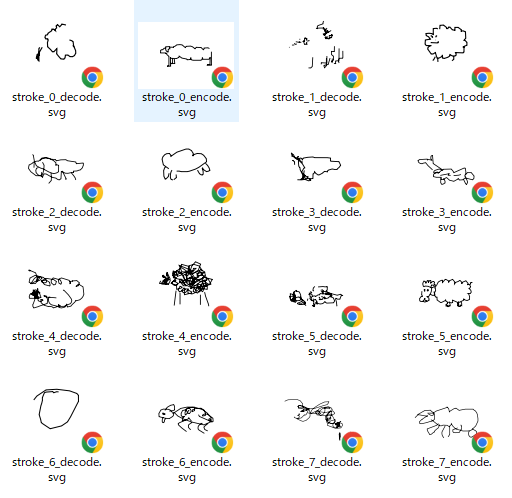
\includegraphics[clip,width=120mm]{ss1000.png}
      \caption{1000 step目での出力}
      \label{fig:result1}
    \end{center}
  \end{figure}

  \begin{figure}[h]
    \begin{center}
      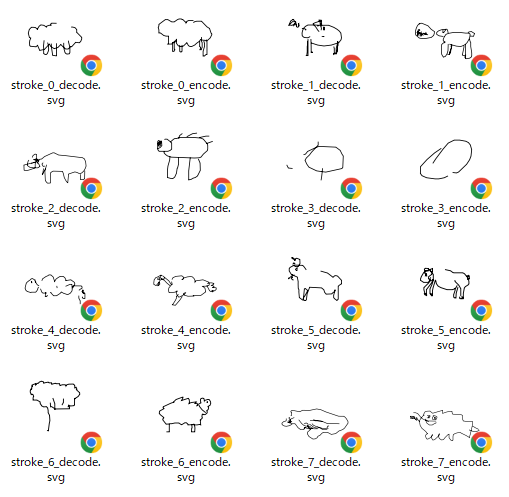
\includegraphics[clip,width=120mm]{ss12000.png}
      \caption{12000 step目での出力}
      \label{fig:result2}
    \end{center}
  \end{figure}

パラメータの学習と結果の出力に関しては問題なく行えることが確認できた.

\newpage
\section{データセットの確認}
データセットに含まれるイラストについて,
絵描き歌に用いるような単純な幾何図形を調査した.

\section{潜在変数(分散表現)の確認}
潜在変数 $z$ の次元数を確認したところ,128 次元であった.
データベースの構築には,
\begin{itemize}
  \item 潜在変数の保存
  \item 潜在変数の類似度比較
\end{itemize}
の 2 つが必要となるため,
まずは類似度比較手法として SSIM を実験できるようにしたい.

\section{今後の予定}
前提段階までは確認できたので,今後は次の類似指標による検索の段階へ移りたい.
いまのところ,予定として以下を考えている.
\begin{itemize}
  \item データベースの作成準備
  \item オリジナルのデータセット作成法の確認
\end{itemize}

% 参考文献リスト
% \bibliographystyle{unsrt}
% \bibliography{ref}
\end{document}
